\documentclass{article}
\usepackage{amsmath,amsthm,amssymb}
\usepackage[T1,T2A]{fontenc}
\usepackage[utf8]{inputenc}
\usepackage[english,russian]{babel}
\usepackage{graphicx}%Вставка картинок правильная
\usepackage{float}%"Плавающие" картинки
\usepackage{wrapfig}%Обтекание фигур (таблиц, картинок и прочего)
\usepackage[most]{tcolorbox} % для управления цветом
\definecolor{block-gray}{gray}{0.95} % уровень прозрачности (1 - максимум)
\newtcolorbox{conclusion}{colback=block-gray,boxrule=0pt,boxsep=0pt} % настройки области с изменённым фоном
\begin{document}
\title{Записи о проделанной работе}
\author{Е.С. Яковлев}
\date{\today}
\maketitle
	\subsection*{1. Найти функицю, которая на $+ \infty$ растёт как линейная функиция, а на $- \infty$ ведёт себя как константа}
	Путём долгих изысканий, я нашёл следующую функцию:
	\fbox{$f(x) = \frac{x^3}{x^2 + e^{-x}}$}
	\\
	Проверим её на соответсвие заданным условиям:
	\begin{itemize}
		\item 	наклонная асимптота на $+ \infty$:
		\begin{gather*}
			\lim_{x\to + \infty} \frac{f(x)}{x} = \lim_{x\to + \infty} \frac{x^3}{x(x^2 + e^{-x})}=\lim_{x\to + \infty} \frac{x^2}{x^2 + e^{-x}}=\lim_{x\to + \infty} \frac{1}{1 + \frac {e^{-x}}{x^2}}=\frac{1}{\lim_{x\to + \infty} \left( 1 + \frac {e^{-x}}{x^2}\right) } =\nonumber \\ =\frac{1}{\lim_{x\to + \infty} \left( 1 + \frac {e^{-x}}{x^2}\right) } = \frac{1}{1 + \lim_{x\to + \infty} \left(\frac {1}{x^2 \cdot e^{x}}\right) } = \frac{1}{1 + \frac{1}{\infty} } = \frac{1}{1 + 0} = 1 \in R
			\end{gather*}
				\item 	поведение константы на $- \infty$:
			\begin{gather*}
			\lim_{x\to + \infty} \frac{f(x)}{x} = \lim_{x\to - \infty} \frac{x^3}{x(x^2 + e^{-x})}=\lim_{x\to - \infty} \frac{x^2}{x^2 + e^{-x}}=\lim_{x\to - \infty} \frac{1}{1 + \frac {e^{-x}}{x^2}}=\frac{1}{\lim_{x\to - \infty} \left( 1 + \frac {e^{-x}}{x^2}\right) } =\nonumber \\ =\frac{1}{\lim_{x\to - \infty} \left( 1 + \frac {e^{-x}}{x^2}\right) } = \frac{1}{1 + \lim_{x\to - \infty}\left( \frac {e^{-x}}{x^2}\right) } = \frac{1}{1 + \infty } = \frac{1}{+\infty} = 0 \in R
			\end{gather*}
	\end{itemize}
	Таким образом, у заданной функции $f(x) = \frac{x^3}{x^2 + e^{-x}}$ есть две асимптоты: на $+\infty$ это прямая вида $y = 1 \cdot x + b$, на $-\infty$ это горизонтальная прямая $y = 0$.
	\begin{figure}[h]
		\centering
		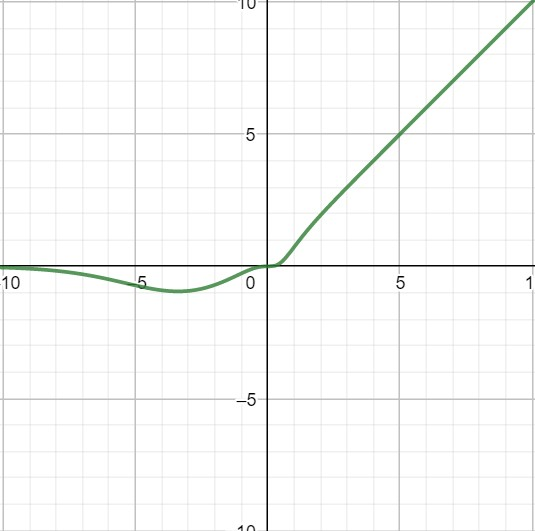
\includegraphics[width=0.5\linewidth]{assets/plot_task_1.jpg}
		\caption{первый вариант: $f(x) = \frac{x^3}{x^2 + e^{-x}}$}
		\label{fig:mpr}
	\end{figure}
	\null\newpage
	\textbf{P.S.}
	В работе будем рассматривать функцию $f(x) = ln(e^x + 1)$.
	\begin{figure}[h]
		\centering
		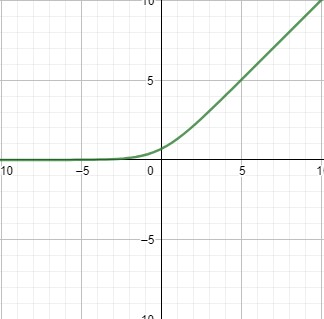
\includegraphics[width=0.5\linewidth]{assets/plot_task_2.jpg}
		\caption{второй вариант: $f(x) = ln(e^x + 1)$}
		\label{fig:mpr}
	\end{figure}
	\null\newpage
	\subsection*{2. Исследовать случай для общества, состоящего только из эгоистов}
	Будем исследовать общество эгоистов, для которого гененрируются случайные предложения с номральным распределением $N\left( \mu = -0.3, \sigma = 10\right)$.\\
	Приведём некоторые параметры модели:
		\begin{itemize}
			\item колличество человек: 300
			\item порог приянтия решения варьируем в промежутке $\left[ 0.4, 0.6\right] $ - берём 100 значений из диапазона
			\item колличество гененрируемых предложений: 100 
			\item генерируем начальные значения капиталов как случайные числа с нормальным распределением $N\left( \mu = -0.3, \sigma = 10\right)$
		\end{itemize}
	 \begin{figure}[h]
	 	\centering
	 	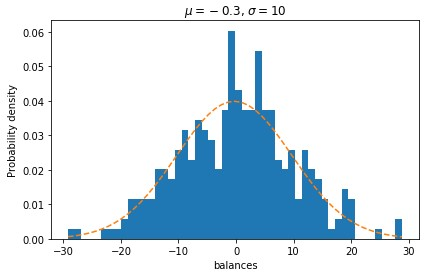
\includegraphics[width=0.8\linewidth]{assets/balances_distribution.jpg}
	 	\caption{нормальное распределение начальных капиталов эгоистов}
	 	\label{fig:mpr}
	 \end{figure}
 Приращение капитала эгоистов будем считать как \fbox{$d_{i} = c_i \cdot (\frac{a}{|\mu|} \cdot f(C_i) + 1)$}, где \fbox{$f(C_i) = ln(e^{C_i} + 1)$}\\
	Рассмотрены три случая:
		\begin{itemize}
			\item $a = 0.1$
			\item $a = 0.5$
			\item $a = 0.9$ 
		\end{itemize}
	\begin{figure}[H]
		\begin{minipage}[h]{0.49\linewidth}
			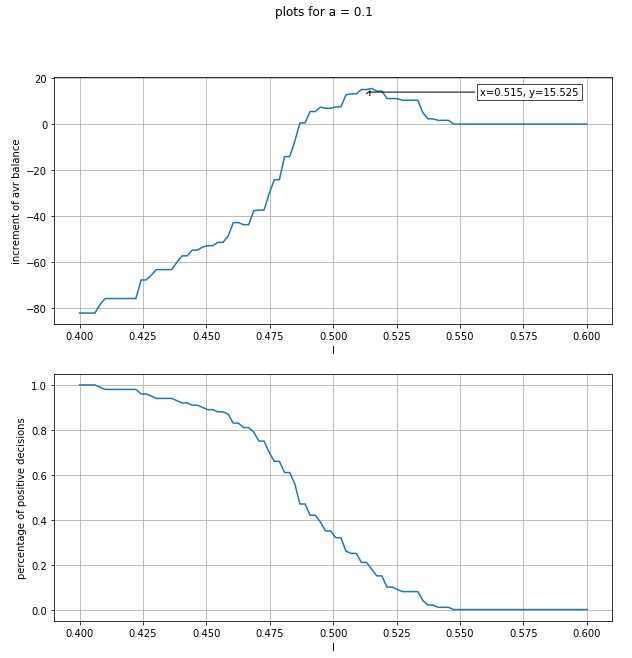
\includegraphics[width=1.0\linewidth]{assets/plot_a01.jpg}
		\end{minipage}
		\hfill
		\begin{minipage}[h]{0.49\linewidth}
			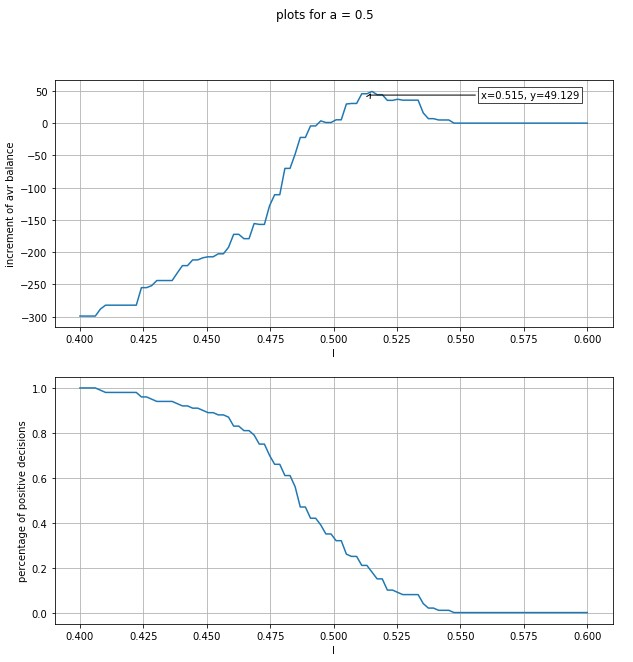
\includegraphics[width=1.0\linewidth]{assets/plot_a05.jpg}
		\end{minipage}
		\hfill
		\begin{minipage}[h]{0.49\linewidth}
			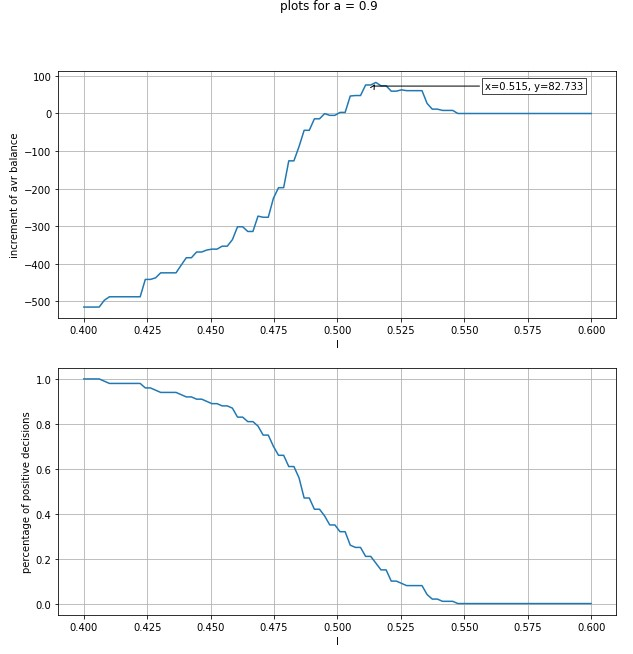
\includegraphics[width=1.0\linewidth]{assets/plot_a09.jpg}
		\end{minipage}
	\end{figure}
Прогнал эту программу на своей функции, которая входит в функцию приращения капитала $f(x) = \frac{x^3}{x^2 + e^{-x}}$ также для трёх значений параметра a:
\begin{itemize}
	\item $a = 0.1$
	\item $a = 0.5$
	\item $a = 0.9$ 
\end{itemize}
\begin{figure}[H]
	\begin{minipage}[h]{0.48\linewidth}
		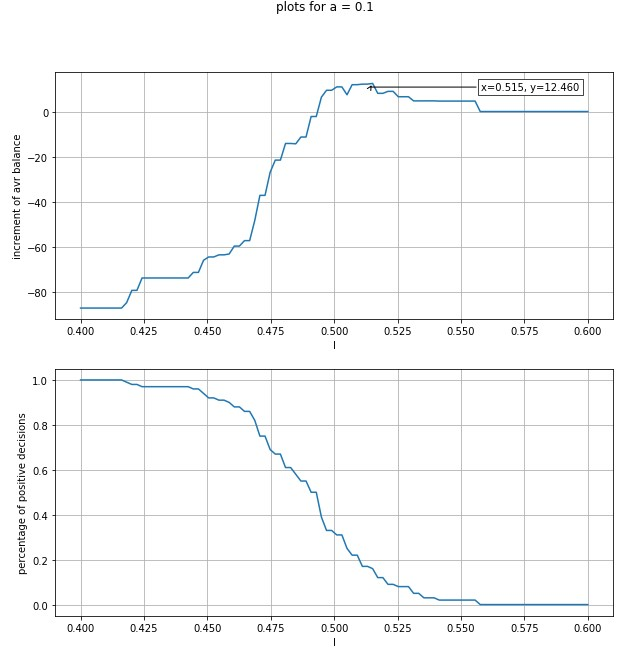
\includegraphics[width=1.0\linewidth]{assets/plot_a01_v2.jpg}
	\end{minipage}
	\hfill
	\begin{minipage}[h]{0.48\linewidth}
		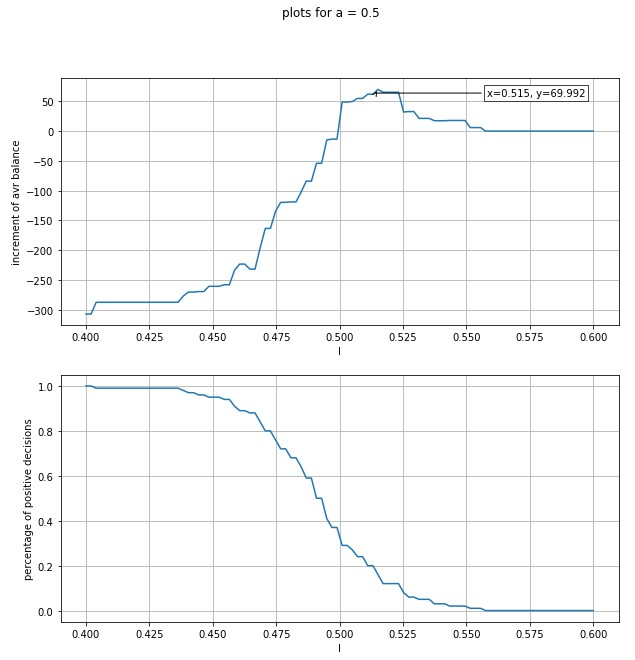
\includegraphics[width=1.0\linewidth]{assets/plot_a05_v2.jpg}
	\end{minipage}
	\hfill
	\begin{minipage}[h]{0.48\linewidth}
		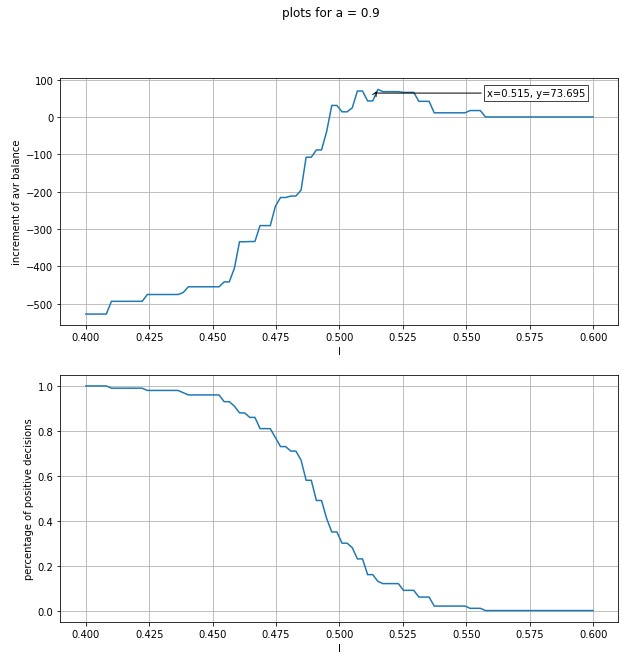
\includegraphics[width=1.0\linewidth]{assets/plot_a09_v2.jpg}
	\end{minipage}
\end{figure}
Графики получились примерно такие же, как и для функции\\
 $f(x) = ln(e^x + 1)$.\\
 \begin{conclusion}
 \textbf{Что можно заметить:}
 	\begin{itemize}
 	\item график зависимости СПК от l достигают своего максимума при одинаковых значениях $l = 0.515$ - программа для случая с функцией $f(x) = ln(e^x + 1)$ и $f(x) = \frac{x^3}{x^2 + e^{-x}}$ работала на разных начальных данных: на разных предложениях и разных начальных балансах 
 \end{itemize}
\end{conclusion}
\null\newpage
\subsection*{3. Зависимость оптимального порога принятия решения $l$ от $\mu$}
	\textbf{Первая итерация}
	\begin{itemize}
	\item $\mu_{min} = -10$, $\mu_{max} = 10$ 
	\item колличество перебирвемых значений $\mu$: 10 
	\item будем рассматривать зависимость $l_{optimal}\left( \mu \right) $ при $a = 0.5$
	\end{itemize}
\begin{figure}[H]
	\centering
	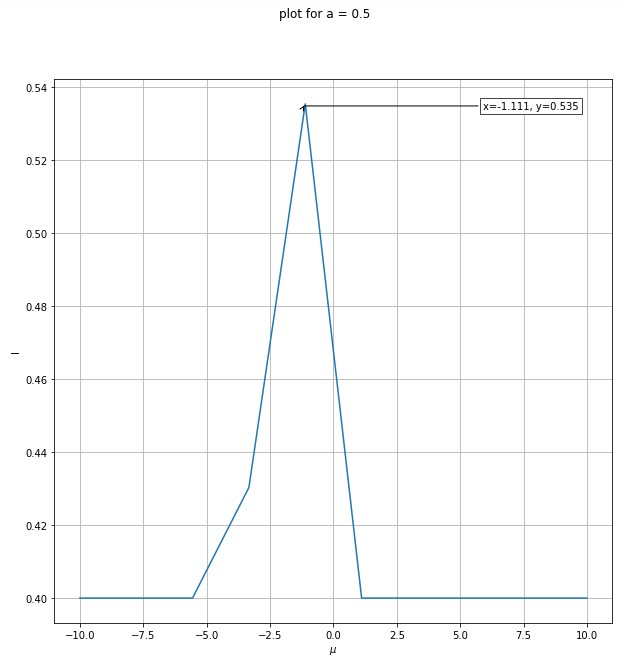
\includegraphics[width=0.7\linewidth]{assets/plot_mu_l.jpg}
	\caption{график $l_{optimal}(\mu)$}
	\label{fig:mpr}
\end{figure}
\textbf{Вторая итерация: увеличенный масштаб в области "горба"}
	\begin{itemize}
	\item $\mu_{min} = -6.0$, $\mu_{max} = 2.5$ 
	\item колличество перебирвемых значений $\mu$: 10 
	\item будем рассматривать зависимость $l_{optimal}\left( \mu \right) $ при $a = 0.5$
\end{itemize}
\begin{figure}[H]
	\centering
	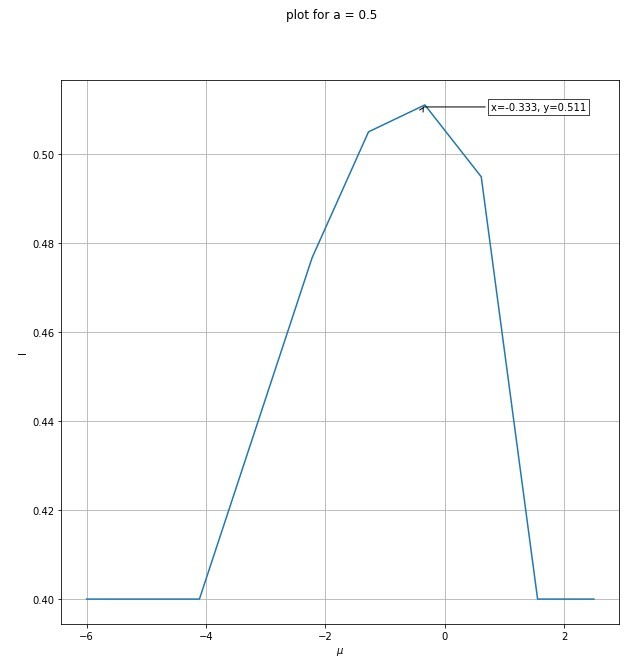
\includegraphics[width=0.7\linewidth]{assets/plot_mu_l_details.jpg}
	\caption{график $l_{optimal}(\mu)$}
	\label{fig:mpr}
\end{figure}
\begin{conclusion}
\textbf{Что можно заметить:}
\begin{itemize}
	\item Мы задаём начальные капиталы эгоистов в обществе как случайные величины с нормальным распределением $N\left(\mu, \sigma \right) $, где $\mu = -0.3$, а $\sigma = 10$
	\item максимум на графике, как можно видеть, достигается при \\ $\mu = -1.017$ и $l_{optimal} = 0.537$
\end{itemize}
\end{conclusion}
\null\newpage
\subsection*{4. Общество эгоистов с одинаковыми начальными \\ капиталами}
	Рассмотрим несколько случаев одинаковых начальных капиталов для всех эгоистов:
	\begin{itemize}
		\item начальный капитал каждого эгоиста принимает одно из значений:\\ -100, -5, 0, 5, 100
		\item случайные числа, которыми заполняются предложения для общества, соответсвуют нормальному распределению $N\left(\mu, {\sigma}^2 \right) $: $\mu = 0.3$, $\sigma = 10$
	\end{itemize}
\begin{figure}[H]
	\begin{minipage}[h]{0.49\linewidth}
		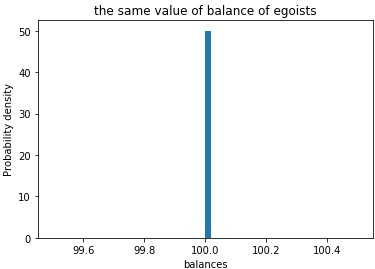
\includegraphics[width=1.0\linewidth]{assets/same_value_distribution_example.jpg}
		\caption{распределение капиталов \newline эгоистов: у всех эгоистов одинаковый капитал}
\end{minipage}
	\hfill
	\begin{minipage}[h]{0.49\linewidth}
		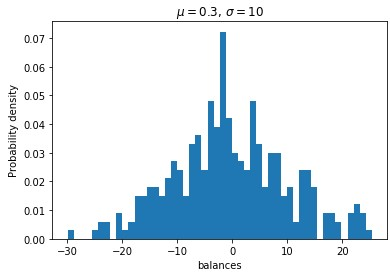
\includegraphics[width=1.0\linewidth]{assets/suggestion_distribution_example.jpg}
		\caption{нормальное распределение случайных чисел в предложениях для общества}
	\end{minipage}
\end{figure}
\null\newpage
\begin{figure}[H]
	\begin{minipage}[h]{0.49\linewidth}
		\centering
		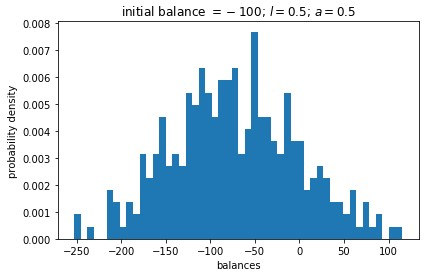
\includegraphics[width=1.0\linewidth]{assets/init_balance_minus_100.jpg}
		конечное распределение капиталов \newline при $balance_{init} = -100$
	\end{minipage}
	\hfill
	\begin{minipage}[h]{0.49\linewidth}
		\centering
		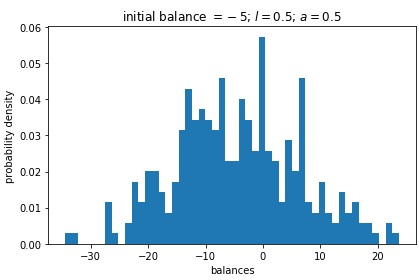
\includegraphics[width=1.0\linewidth]{assets/init_balance_minus_5.jpg}
		конечное распределение капиталов \newline при $balance_{init} = -5$
	\end{minipage}
\end{figure}
\begin{figure}[H]
		\centering
		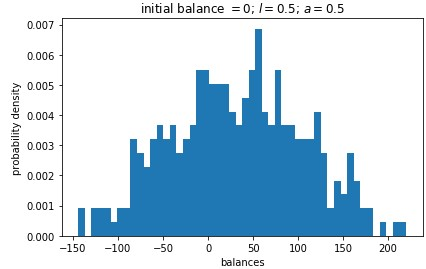
\includegraphics[width=0.5\linewidth]{assets/init_balance_0.jpg}
		\begin{center}
		конечное распределение капиталов при $balance_{init} = 0$
		\end{center}
\end{figure}
\begin{figure}[H]
	\begin{minipage}[h]{0.49\linewidth}
		\centering
		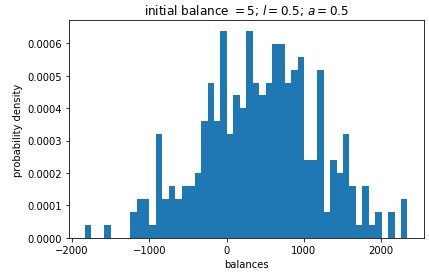
\includegraphics[width=1.0\linewidth]{assets/init_balance_5.jpg}
		конечное распределение капиталов \newline при $balance_{init} = 5$
	\end{minipage}
	\hfill
\begin{minipage}[h]{0.49\linewidth}
	\centering
	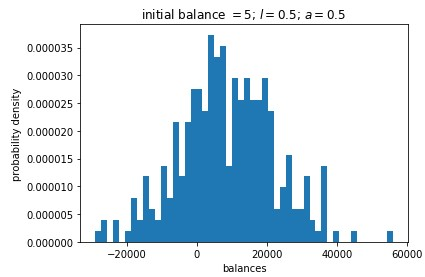
\includegraphics[width=1.0\linewidth]{assets/init_balance_100.jpg}
	конечное распределение капиталов \newline при $balance_{init} = 100$
\end{minipage}
\end{figure}
\null\newpage
Снова зададим эгоистам в обществе одинаковые начальные капиталы: пусть $balance_{init} = 5$. Рассмотрим зависимость СПК от порогового значения принятия решения $l$.
\begin{figure}[H]
	\centering
	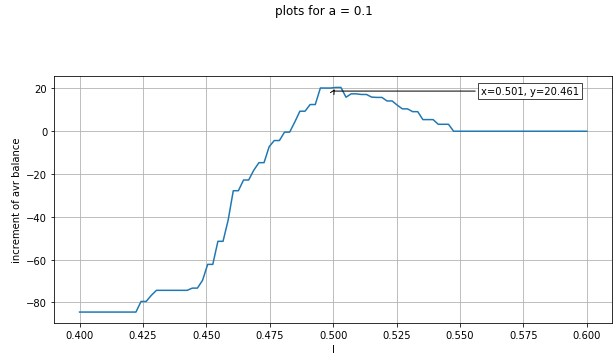
\includegraphics[width=0.6\linewidth]{assets/one_value_distribution/plot_a01.jpg}
	\caption{$ABG(l)$ при $balance_{init} = 5$ и $a = 0.1$}
\end{figure}

\begin{figure}[H]
	\centering
	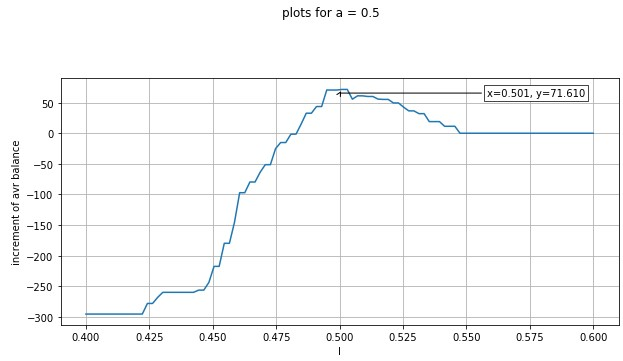
\includegraphics[width=0.6\linewidth]{assets/one_value_distribution/plot_a05.jpg}
	\caption{$ABG(l)$ при $balance_{init} = 5$ и $a = 0.5$}
\end{figure}

\begin{figure}[H]
	\centering
	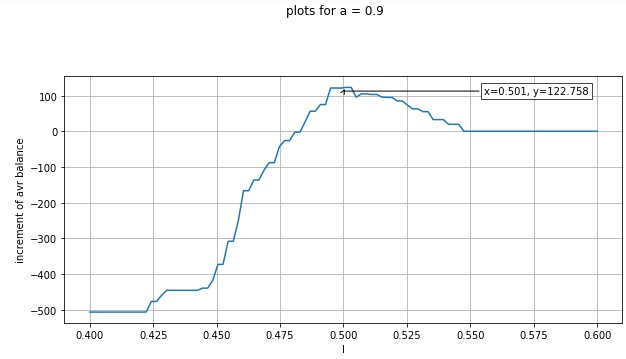
\includegraphics[width=0.6\linewidth]{assets/one_value_distribution/plot_a09.jpg}
	\caption{$ABG(l)$ при $balance_{init} = 5$ и $a = 0.9$}
\end{figure}

\begin{figure}[H]
	\centering
	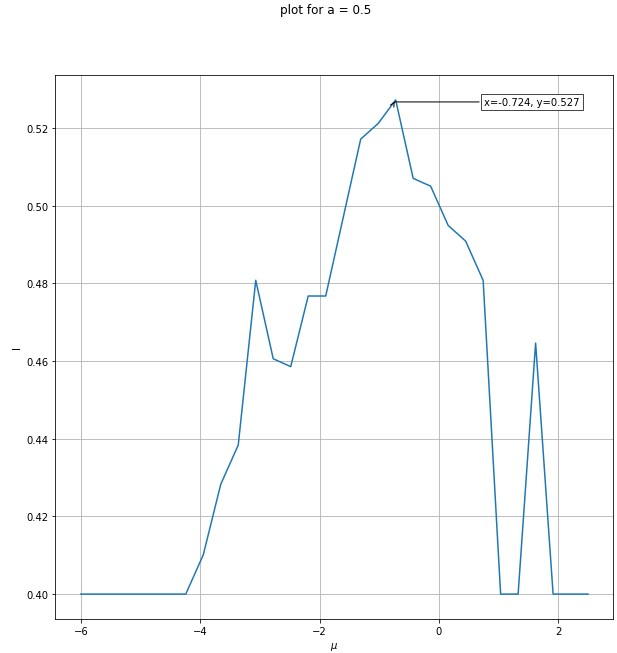
\includegraphics[width=0.7\linewidth]{assets/one_value_distribution/plot_mu_l_details.jpg}
	\caption{Зависимость $l_{optim}(\mu)$ при $a = 0.5$ и при одинаковых значениях $balance_{init} = 5$}
\end{figure}
\end{document}